
\begin{refsection}
\startcontents[chapters]
\chapter{Monte Carlo Methods \& optimization}\label{ch:MonteCarlo-methods--optimization}
	
\printcontents[chapters]{}{1}{}
\section{Generating Random Variables}\label{ch:MonteCarlo-methods--optimization:sec:generateRN}\index{random number generation}
\begin{mdframed}
	\textbf{Assumption:}we are able to generate random variables with uniform distribution.
\end{mdframed}


\subsection{Inverse transform method}\label{ch:MonteCarlo-methods--optimization:sec:inversetransformrandomnumbergeneration}
\begin{method}[inverse transform method]
	Assume the random variable we want to generate has a cdf $F(x)$ strictly increasing. Then we have
	\begin{enumerate}
		\item Generate $X\sim U([0,1])$
		\item Set $Y = F^{-1}(x)$
	\end{enumerate}
	then $Y$ has cdf $F(x)$.
\end{method}

\begin{remark}\hfill
	\begin{itemize}
		\item If $F(x)$ is not strictly increasing, then we define $F^{-1}(u) = \inf\{F^{-1}(x > u)\}$
		\item This method is useful usually when we have explicitly expression for $F^{-1}$.
		\item For Gaussian random variable, we usually use Box-Muller transform.
		\item For discrete distribution, we can also use this method since $F^{-1}$ is easy to construct.
	\end{itemize}
\end{remark}


\begin{remark}[Box muller transformation method for generating standard normal]
To generate standard normal variable, we can use Box-Muller transformation, see \autoref{ch:theory-of-statistics:th:BoxMullerTransformation}.	
\end{remark}

\begin{example}
Given a random variable $U$ drawn from the uniform distribution in the interval $(0,1]$, the random variable
$$X = \mu - b~sgn(U-0.5)\ln (1-2\abs{U-0.5})$$	
will have Laplace distribution with parameter $(\mu,b)$.

Note that we have used the fact that the inverse cdf of Laplace distribution is given by(\autoref{ch:theory-of-statistics:th:PropertiesOfLaplaceDistribution}):
$$F^{-1}(p) = \mu - b\cdot sgn(p-0.5)\ln(1-2\abs{p-0.5}).$$
\end{example}

\begin{lemma}[generalized inverse transform method]\label{ch:MonteCarlo-methods--optimization:th:GeneralizedInverseTransformMethod}
Let $X$ be a random variable with cdf $F_X$. We can use the following ways to sample $X$:
\begin{itemize}
	\item Let $U\sim U([0,1])$ be an uniform random variable. Then the transformed random variable  $W = F_X^{-1}(U)$ has the same distribution of $X$.
	\item  Let $Z\sim N(0,1)$ be a standard normal random variable with cdf $\phi$. Then transformed random variable $W=F_X^{-1}(\phi(Z))$ has the same distribution of $X$.
	\item  Let $Y$ be a normal random variable with cdf $F_Y$. Then transformed random variable $W = F_X^{-1}(F_Y(Y))$ has the same distribution of $X$.
\end{itemize}	
\end{lemma}
\begin{proof}
(1) $$F_W(w) = Pr(F_X^{-1}(U) < w) = Pr(U < F_X(w)) = F_X(w).$$
(2) 
\begin{align*}
F_W(w) &= Pr(F_X^{-1}(\phi(Z)) < w) \\
&= Pr(\phi(Z) < F_X(w))  \\
&= Pr(Z < \phi^{-1}(F_X(w))) \\
&= \phi\circ \phi^{-1}(F_X(w))) \\
&= F_X(w)
\end{align*}
(3) \begin{align*}
F_W(w) &= Pr(F_X^{-1}(F_Y(Y)) < w) \\
&= Pr(F_Y(Y) < F_X(w))  \\
&= Pr(Y < F_Y^{-1}(F_X(w))) \\
&= F_Y\circ F_Y^{-1}(F_X(w))) \\
&= F_X(w)
\end{align*}
\end{proof}

\subsection{Box-Muller method for standard normal random variable}



\begin{lemma}[Box Muller method for standard normal random variable]\autoref{ch:theory-of-statistics:th:BoxMullerTransformation}Suppose we have $U_1,U_2$ being independent uniform on $[0,1]$.
Define $$X=\sqrt{-2\ln(1-U_2)}\cos(2\pi U_1), Y=\sqrt{-2\ln(1-U_2)}\sin(2\pi U_1).$$
Then
  $X,Y\sim N(0,1)$ and $X,Y$ be independent. 
\end{lemma}
\begin{proof}
See \autoref{ch:theory-of-statistics:th:BoxMullerTransformation}.
\end{proof}

\subsection{Acceptance-rejection method}
\iffalse
\begin{theorem}[The fundamental theorem of random number generation]\index{The fundamental theorem of random number generation}
	Simulating $X\sim f(x)$ is equivalent to simulating uniform distribution
	$$(X,U)\sim (x,u)$$
	
\end{theorem}



Suppose $X$ has pdf $p(x)$, and $p(x)$ is bounded as $0\leq p(x) < d$, with support on $[a,b]$. To generate $X$, we have\cite{Holmes-Cerfon2015applied}
\begin{enumerate}
	\item generate $X'\sim U([a,b]),Y\sim U([0,d])$
	\item If $Y \leq p(X')$, \textbf{accept}, $X=X'$
	\item otherwise, reject, go to step 1.
\end{enumerate}
Proof: The joint distribution of $(X',Y)$ (if accepted)is a indicator $I_A$ function on $[a,b]\times[0,d]$ with the set $A=\{(x,y):x\in[a,b],0\leq y<p(x)\}$. The marginal distribution of $p(X')=\int_0^d I_A(x,y)dy = \int_0^{p(x)} dy = p(x)$

\begin{remark}\hfill
	\item this method is inefficient if area of $A$ is very small (for example, $[a,b]$ is very large, $p(x)$ has large peaks etc.)
\end{remark}
\fi

\begin{algorithm}[H]
	\SetAlgoLined
	\KwIn{  the proposal distribution $q(x)$, the target distribution $p(x)$, and $M = \sup_x p(x)/q(x)$}
	Sample $x\sim q(x)$ and $u \sim U([0,1])$\\
	If $u < \frac{p(x)}{Mq(x)}$, then accept $x$, otherwise reject.\\
	Goto step 1.\\
	\KwOut{The sample $x$}
	\caption{Accept-Reject algorithm }
\end{algorithm}

\begin{remark}\hfill
	\begin{itemize}
		\item Reference \cite{andrieu2003introduction}\cite[272]{hoggintroduction}.
		\item The $q(x)$ and $p(x)$ are required to have the same support.
	\end{itemize}
\end{remark}

\begin{example}
	Suppose we want to generate 
	$p(x) = \frac{2}{\sqrt{2\pi}} e^{-x^2/2},x\geq 0$. We can choose $q(x) = e^{-x},x\geq 0$. Then 
	$$M = \frac{p(x)}{q(x)} = e^{x-x^2}\sqrt{2/\pi}$$
	will achieve maximum value at $x=1$. 
	Then the thresholding value is $$\frac{p(x)}{q(x)M} = e^{(y-1)^2/2}.$$
\end{example}


\begin{lemma}[probability of acceptance]
	In the Rejection algorithm, the probability to accept is $1/M$, and the average step needed to generate one accepted random sample $x$ is $M$.
\end{lemma}
\begin{proof}
	$$f(X = x \cap accept) = q(x)\frac{p(x)}{Mq(x)} = p(x)/M $$
	$P(accept) = \int f(X = x \cap accept) dx =1/M$.
	This is a geometric distribution with parameter $1/M$, which has an expected number of $M$.
\end{proof}


\begin{remark}[implication]
	The larger $M$, the lower the acceptance ratio and the simulation efficiency.	
\end{remark}

\begin{lemma}[correctness of algorithm]
	The Accept-Reject algorithm will generate random number $X$ with $p(x)$.
\end{lemma}
\begin{proof}
	\begin{align*}
	P[X \leq x | accept] &= P[X\leq x \cap U < \frac{p(x)}{Mq(x)}]/P[U < \frac{p(x)}{Mq(x)}]\\
	&=\frac{\int_{-\infty}^x \frac{p(y)}{Mq(y)}q(y)dy}{\int_{-\infty}^\infty \frac{p(y)}{Mq(y)}q(y)dy}\\
	& = F_X(x)
	\end{align*}
\end{proof}

\subsection{Composition approach}
\begin{lemma}
	Suppose we want to generate a random variable $X$ with cdf $F_X$. If we can find decomposition such that
	$$F_X(x) = \sum_{i=1}^{N} p_i F_i(x),$$
	where $p_i\geq 0, \forall i, p_1+p_2+ \cdots + p_N = 1$.
	Or equivalently, 
	$$f_X(x) = \sum_{i=1}^{N} p_i f_i(x).$$
	
	Then we can generate $X$ via the following procedures:
	\begin{itemize}
		\item Generate a positive random integer $J$ such that $Pr(J=j) = p_j$.
		\item Return $X$ with cdf $F_j$.
	\end{itemize}
\end{lemma}
\begin{proof}
For a given fixed $x$, we have
\begin{align*}
Pr(X < x) &= \sum_{j=1}^{N} Pr(X\leq x|J=j)Pr(J=j) \\
&=\sum_{j=1}^{N} Pr(X\leq x|J=j)p_j \\
&=\sum_{j=1}^{N} F_j(x)p_j \\
&=F_X(x)
\end{align*}	
where use the law of total probability in the first line ( \autoref{ch:theory-of-probability:th:lawoftotalprobability})
\end{proof}

\begin{example}
Suppose we want to generate a random variable $X$ with density given by
$$f(x) = \begin{cases*}
x+1, -1\leq x \leq 0\\
-x+1, 0\leq x\leq 1\\
0, otherwise
\end{cases*}.$$	
We can have the decomposition as
\begin{align*}
f(x) &= (x+1) \bm{1}_{[-1,0]}(x) + (-x+1)\bm{1}_{[0,1]}(x) \\
&= 0.5 \times 2(x+1) \bm{1}_{[-1,0]}(x) + 0.5\times 2(-x+1)\bm{1}_{[0,1]}(x) \\
&= p_1f_1(x) + p_2f_2(x)
\end{align*}
where $p_1=p_2=0.5$ and $f_1 = 2(x+1) \bm{1}_{[-1,0]}(x)$ and $f_2=2(-x+1)\bm{1}_{[0,1]}(x)$.

We can integrate $f_1$ and $f_2$ to get
$$F_1(x) = x^2+2x+1, F_2(x) = -x^2+2x,$$
and
$$F_1^{-1}(U)=\sqrt{U}-1, F_2^{-1}(U) = 1 - \sqrt{1-U}.$$

Eventually, we can use the following algorithm to generate the desired $X$:
\begin{itemize}
	\item Generate $U_1,U_2 \sim U(0,1)$ independently.
	\item If $U_1<0.5$, return $X = \sqrt{U_2}-1$; else return $X = 1-\sqrt{1-U_2}$.
\end{itemize}

\end{example}


\begin{example}
	Suppose we want to generate a random variable $X$ with density given by
	$$f(x) = \begin{cases*}
	2-a-2(1-a), 0\leq x \leq 1\\
	0, otherwise
	\end{cases*}.$$	
	We can have the decomposition as
	\begin{align*}
	f(x) &= a \bm{1}_{[0,1]}(x) + (1-a)2(1-x)\bm{1}_{[0,1]}(x) \\
	&= p_1f_1(x) + p_2f_2(x)
	\end{align*}
	where $p_1=a,p_2=1-a$ and $f_1 = \bm{1}_{[0,1]}(x)$ and $f_2=(1-a)2(1-x)\bm{1}_{[0,1]}(x)$.
	
	We can integrate $f_1$ and $f_2$ to get
	$$F_1(x) = x, F_2(x) = -x^2+2x,$$
	and
	$$F_1^{-1}(U)=U, F_2^{-1}(U) = 1 - \sqrt{1-U}.$$
	
	Eventually, we can use the following algorithm to generate the desired $X$:
	\begin{itemize}
		\item Generate $U_1,U_2 \sim U(0,1)$ independently.
		\item If $U_1<a$, return $X = U_2$; else return $X = 1-\sqrt{1-U_2}$.
	\end{itemize}
	
\end{example}


\subsection{Generate discrete random variables}


\subsubsection{Generate single discrete random variables}

\begin{lemma}[generate discrete random variable]
	Assume we are given the  distribution function of random variable $X$,
	$$Pr(X=x_i) = p_{i}, i=1,2,...,n.$$
	We can divide the interval $[0,1]$ into $n$ buckets of
	$$[0,p_1),[p_1,p_1+p_2),...,[\sum_{i=1}^{n-1} p_i,1).$$
	Then we generate a uniform random variable $U$: if $U$ falls into bucket $i$, we will produce $X = x_i$.
\end{lemma}
\begin{proof}
It is easy to see that the probability for us to sample $X=x_i$ is $p_i$.
\end{proof}

\subsubsection{Generate correlated discrete random variables}

\begin{lemma}[generate a pair of random variables with arbitrary joint distribution]\label{ch:MonteCarlo-methods--optimization:th:generatePairRandomVariablesWithArbitraryJointDistribution}
	Assume we are given the joint distribution function for random variable $X$ and $Y$ as
	$$Pr(X=x, Y=y) = p_{xy}.$$
	
	Then we have
	$$Pr(X = x) = \sum_y p_{xy}$$
	which can be used to generate $X$; and
	$$Pr(Y=y|X=x)= p_{xy}/Pr(X=x)$$	
	which can be used to generate $Y$ conditioned on the generated $X$.
\end{lemma}


\begin{lemma}[generate two correlated random variables with arbitrary joint distribution]
Assume we are given the marginal distribution function for random variable $X$ and $Y$ as
$$Pr(X=x) = p_x, Pr(Y=y) = p_y.$$

Denote the joint distribution by $Pr(X=x,Y=y) = a_{xy}$.
Then we can solve a joint distribution with correlation $\rho$ via the following equation system
\begin{align*}
\sum_x a_{xy} &= p_y, \forall y \\
\sum_y a_{xy} &= p_x, \forall x \\
\sum_{x,y} a_{xy} &= 1\\
\frac{E[XY]-E[X]E[Y]}{\sqrt{E[X^2]-E[X]^2}\sqrt{E[Y^2]-E[Y]^2}} &=\rho 
\end{align*}

The solved the joint distribution can be used to generate correlated random variables via \autoref{ch:MonteCarlo-methods--optimization:th:generatePairRandomVariablesWithArbitraryJointDistribution}.	
\end{lemma}
\begin{proof}
The equation system is constructed by requiring the satisfaction of margins, sum-to-unit, and correlation.
\end{proof}

\begin{remark}[existence and uniqueness of joint distribution]
Note that the joint distribution satisfying the specified correlation condition might not exist; even exists, that might not be unique. However, each joint distribution satisfying above condition will enable us to get the random variables with desired correlation.
\end{remark}


\begin{lemma}[generate two correlated Bernoulli random variables]
Suppose we want to generate two Bernoulli random variable $X$ and $Y$ with coefficients $p$ and $q$, respectively. Further we want the two random variables have correlation coefficient $\rho$. That is,
$$Pr(X=1) = p, Pr(Y=1) = q.$$

Then the joint distribution for $(X,Y)$ can be uniquely determined, and the correlated random variables $X$ and $Y$ can be generated using \autoref{ch:MonteCarlo-methods--optimization:th:generatePairRandomVariablesWithArbitraryJointDistribution}.
\end{lemma}
\begin{proof}
Note that $$\rho = \frac{E[XY] - E[X]E[Y]}{\sqrt{E[X^2]-E[X]^2}\sqrt{E[Y^2]-E[Y]^2}} = \frac{Pr(X=1,Y=1)-pq}{\sqrt{p(1-p)}\sqrt{q(1-q)}}.$$

Denote the joint distribution $$Pr(X=i,Y=j) = a_{ij},i=0,1;j=0,1,$$
then we can solve the joint distribution via	
\begin{align*}
a_{10} + a_{11} &= p\\
a_{01} + a_{11} &= q\\
a_{11} &= pq + \rho \sqrt{p(1-p)q(1-q)} \\
a_{00} + a_{01} + a_{10} + a_{11} &= 1
\end{align*}
\end{proof}


\subsection{Generate dependent continuous random variables}

\subsubsection{General joint distribution}
\begin{lemma}[generate dependent continuous random variables from joint distribution]
Suppose we know the entire joint distribution $F_X$ for a random vector $X=(X_1,X_2,...,X_N)$. 

Then we can use the following algorithm to generate a random vector $X=(X_1,X_2,...,X_N)$:
\begin{itemize}
	\item Generate $X_1$ from the marginal distribution $F_{X_1}$ via inverse transform(\autoref{ch:MonteCarlo-methods--optimization:sec:inversetransformrandomnumbergeneration}).
	\item Generate $X_2$ from the conditional distribution $F_{X_2|X_1}$via inverse transform.
	\item Generate $X_3$ from the conditional distribution $F_{X_3|X_1,X_2}$via inverse transform.
	\item $\cdots$
	\item Generate $X_N$ from the conditional distribution $F_{X_N|X_1,X_2,...,X_{N-1}}$ via inverse transform.
	\item Finally,  return $X=(X_1,X_2,...,X_N)$.
\end{itemize}
\end{lemma}

\subsubsection{Multivariate normal distribution}
\begin{lemma}[generate multivariate normal random vector]\label{ch:MonteCarlo-methods--optimization:th:generateMultivariateNormalRandomVector}
Suppose we want to generate a random vector $X=(X_1,X_2,...,X_n)\sim MN(\mu, \Sigma)$. We can use the following algorithm to generate $X$:
\begin{itemize}
	\item Generate $Z_1,Z_2,...,Z_n$ as iid $N(0,1)$, and let $Z = (Z_1,Z_2,...,Z_n).$
	\item Return $X= \mu + CZ$, where $C$ is the Cholesky decomposition of $\Sigma$ such that $\Sigma = CC^T$.
\end{itemize}	
\end{lemma}
\begin{proof}
It can be showed via \autoref{ch:theory-of-statistics:th:affinetransformmultivariatenormal} that
$$X\sim MN(\mu, \Sigma).$$
\end{proof}


\subsubsection{Multivariate log-normal distribution}
\begin{lemma}[generate multivariate lognormal random vector]
Suppose we want to generate a random vector $X=(X_1,X_2,...,X_n)\sim LMN(\mu, \Sigma)$. We can use the following algorithm to generate $X$:
\begin{itemize}
	\item Generate $Z=(Z_1,Z_2,...,Z_n)$ as $MN(\mu,\Sigma)$ using \autoref{ch:MonteCarlo-methods--optimization:th:generateMultivariateNormalRandomVector}.
	\item Return $X= (\exp(Z_1),\exp(Z_2),...,\exp(Z_n))$.
\end{itemize}	
\end{lemma}
\begin{proof}
See the definition of multivariate lognormal distribution(\autoref{ch:theory-of-statistics:def:multivariateLognormalDistribution}).
\end{proof}

\subsubsection{Multivariate student t distribution}
\begin{lemma}[generate multivariate student t random vector]\label{ch:MonteCarlo-methods--optimization:th:generateMultivariateStudentTRandomVector}
	Suppose we want to generate a random vector $X=(X_1,X_2,...,X_n)\sim t_n(\mu, \Sigma)$. We can use the following algorithm to generate $X$:
	\begin{itemize}
		\item Generate $Z_1,Z_2,...,Z_n$ as iid $N(0,1)$, and let $Z = (Z_1,Z_2,...,Z_n).$
		\item Generate a random $W\sim \chi^2(n)$ independent of $Z$.
		\item Return $X= \mu + \sqrt{\frac{n}{W}}CZ$, where $C$ is the Cholesky decomposition of $\Sigma$ such that $\Sigma = CC^T$.
	\end{itemize}	
\end{lemma}
\begin{proof}
	It can be showed via the definition of multivariate $t$ distribution(\autoref{ch:theory-of-statistics:def:MultivariateTDistribution}) that
$$X = \mu + \sqrt{\frac{n}{W}}CZ,$$
where $W\sim \chi^2(n)$ and $W$ is \textbf{independent} of $Z$,
has a $t_n(\mu,\Sigma)$ multivariate distribution.
\end{proof}


\section{Simulating random processes}

\subsection{Simulating Brownian motion}
\begin{method}[exact simulation one D Brownian motion]\cite[705]{campolieti2016financial}
Let $0=t_0<t_1<...<t_m$ be a set of dates.
\begin{itemize}
	\item We can simulate a standard Brownian motion $W(t)$ on this set of dates using the following procedure:
	\begin{itemize}
		\item set $W(t_0) = 0$.
		\item generate independent $Z_j\sim N(0,1), j=1,2,...,m$.
		\item set $W(t_j) = W(t_{j-1}) + \sqrt{t_j-t_{j-1}}Z,j=1,2,...,m$.
	\end{itemize}
	\item We can simulate a drifting scaled Brownian motion $$W(t;\mu,\sigma,x_0) = x_0+\mu t + \sigma W(t)$$
	using the following procedure:
	\begin{itemize}
		\item set $W(t_0;\mu,\sigma,x_0) = x_0$.
		\item generate independent $Z_j\sim N(0,1), j=1,2,...,m$.
		\item set $W(t_j;\mu,\sigma,x_0) = W(t_{j-1};\mu,\sigma,x_0) + \mu(t_j-t_{j-1})+\sigma\sqrt{t_j-t_{j-1}}Z,j=1,2,...,m$.
	\end{itemize}
\end{itemize}	

Note that the simulated sequence $W(t)$ and $W(t;\mu,\sigma,x_0)$ has the exact distribution desired.
\end{method}


\subsection{Simulating linear arithmetic SDE}

\begin{method}[simulating linear arithmetic SDE]\cite[104]{glasserman2003monte}
Suppose we want to simulate
$$dx(t) = \mu(t)dt + \sigma(t)dW_t, x(0) = x_0.$$
Let $0=t_0<t_1<...<t_m$ be a set of evenly space dates.

We can simulate a standard Brownian motion $W(t)$ on this set of dates using the following procedure:
	\begin{itemize}
		\item start from $i=1$.
		\item $$x(t_{i}) = x_{t_{i-1}} + \mu(t_i)(t_{i}-t_{i-1}) + \sigma(t_i)\sqrt{t_{i}-t_{i-1}}Z$$
		where $Z\sim N(0,1)$.
		\item Set $i=i+1$.
		\item Repeat step (2)(3) until $i=N$.
	\end{itemize}
\end{method}




\subsection{Simulating linear geometric SDE}

\begin{method}[simulating linear arithmetic SDE]\cite[104]{glasserman2003monte}
	Suppose we want to simulate
	$$dx(t)/x(t) = \mu(t)dt + \sigma(t)dW_t, x(0) = x_0.$$
	Let $0=t_0<t_1<...<t_m$ be a set of evenly space dates.
	
	We can simulate a standard Brownian motion $W(t)$ on this set of dates using the following procedure:
	\begin{itemize}
		\item start from $i=1$.
		\item $$x(t_{i}) = x_{t_{i-1}}\exp(  (\mu(t_i) - \frac{1}{2}\sigma(t_i)^2)(t_{i}-t_{i-1}) + \sigma(t_i)\sqrt{t_{i}-t_{i-1}}Z)$$
		where $Z\sim N(0,1)$.
		\item Set $i=i+1$.
		\item Repeat step (2)(3) until $i=N$.
	\end{itemize}
\end{method}



\subsection{Simulation mean-reversion(OU) process}

\begin{method}[simulating a mean-reversion process]\cite[104]{glasserman2003monte}
	Suppose we want to simulate
$$dx(t) = (\theta(t)-kx_t)dt + \sigma(t)dW_t, x(0) = x_0.$$
Let $0=t_0<t_1<...<t_m$ be a set of evenly space dates.

We can simulate a standard Brownian motion $W(t)$ on this set of dates using the following procedure:
\begin{itemize}
	\item start from $i=1$.
	\item $$x(t_{i}) = x_{t_{i-1}} + (\theta(t_{i-1}) - kx(t_{i-1})(t_i-t_{i-1})  + \sigma(t_i)\sqrt{t_{i}-t_{i-1}}Z$$
	where $Z\sim N(0,1)$.
	\item Set $i=i+1$.
	\item Repeat step (2)(3) until $i=N$.
\end{itemize}	
\end{method}




\subsection{Stochastic interpolation}

\subsubsection{Interpolating Gaussian processes}
\begin{method}[interpolating a Gaussian process]
Let $X_t$ be a Gaussian process with mean function $\mu(t)$ and covariance function $cov(t_i,t_j)$. 

Consider a set of time points $t_a<t_1<t_2<... <t_n< t_b$. Suppose we are given $X(t_a)$ and $X(t_b)$ and we want to sample $X(t_1),X(t_2),X(t_3),...,X(t_n)$. 

Construct a conditional mean vector and a conditional covariance matrix  given by$$m = \mu_1 + \Sigma_{12}\Sigma_{22}^{-1}(x_2 - \mu_2), V = \Sigma_{11} - \Sigma_{12}\Sigma_{22}^{-1}\Sigma_{12}^T, $$
where 
\begin{align*}
&\Sigma_{22} = \begin{bmatrix}
Cov(X_1,X_1) & Cov(X_1,X_2) & \cdots & Cov(X_1,X_n)\\ 
Cov(X_2,X_1) & Cov(X_2,X_2) & \cdots & Cov(X_2,X_n)\\ 
\vdots & \cdots & \ddots & \vdots\\ 
Cov(X_n,X_1) & Cov(X_n,X_2) & \cdots & Cov(X_n,X_n) 
\end{bmatrix},\Sigma_{11} = \begin{bmatrix}
Cov(X_a,X_a) & Cov(X_a,X_b) \\
Cov(X_a,X_b) & Cov(X_b,X_b)  
\end{bmatrix}, \\
&\Sigma_{12} = \begin{bmatrix}
Cov(X_a,X_1) & Cov(X_a,X_2) & \cdots & Cov(X_a,X_n) \\
Cov(X_b,X_1) & Cov(X_b,X_2) & \cdots & Cov(X_b,X_n) 
\end{bmatrix}, \mu_2 = \begin{bmatrix}
\mu(t_1)\\
\mu(t_2)\\
\cdots \\
\mu(t_n)
\end{bmatrix},x_2 = \begin{bmatrix}
X_1\\
X_2\\
\cdots \\
X_n
\end{bmatrix},\mu_1 = \begin{bmatrix}
X_a\\
X_b
\end{bmatrix}
\end{align*}
Then we can generate a multivariate Gaussian random variable with mean $m$ and covariance matrix $V$ using \autoref{ch:MonteCarlo-methods--optimization:th:generateMultivariateNormalRandomVector}.	
\end{method}
\begin{proof}

\end{proof}

\subsubsection{Interpolating one Dimensional Brownian motions}
\begin{lemma}[interpolating a standard Brownian motion]
Let $X_t$ be a standard Brownian motion. Consider three time points $t_a<t_1<t_b$. Then conditioning on values of $X(t_a)$ and $X(t_b)$,
$X(t_1)$ is a Gaussian random variable with mean and variance $$\mu = X(t_a) + \frac{t_1-t_a}{t_b-t_a}(X(t_b)-X(t_a)), \sigma^2 = t_1-t_a - \frac{(t_1-t_a)^2}{(t_b-t_a)}.$$
\end{lemma}
\begin{proof}
Note that the random vector $(X(t_a), X(t_1),X(t_b))$ will follow multivariate Gaussian distribution since $X_t$ is a Gaussian process. Conditioning on $X(t_a)$ and $X(t_b)$, $X(t_1)$ is a Gaussian random variable with conditional mean and variance given by(\autoref{ch:theory-of-statistics:th:multivariatenormalconditionaldistribution}) $$\mu=[t_a ~ t_1]\begin{bmatrix}
t_a & t_a\\
t_a & t_b
\end{bmatrix}^{-1}\begin{bmatrix}
X(t_a)\\
X(t_b)
\end{bmatrix} = X(t_a) + \frac{t_1-t_a}{t_b-t_a}(X(t_b)-X(t_a)),$$
and
variance
$$\sigma^2 = t_1 - [t_a ~ t_1]\begin{bmatrix}
t_a & t_a\\
t_a & t_b
\end{bmatrix}^{-1}\begin{bmatrix}
t_a\\
t_1
\end{bmatrix}= t_1-t_a - \frac{(t_1-t_a)^2}{(t_b-t_a)}$$
\end{proof}

\begin{lemma}[interpolating a scaled Brownian motion]
Let $Y_t$ be a Brownian motion. Let $X_t = vt + \sigma Y_t$. Consider three time points $t_a<t_1<t_b$. Then conditioning on values of $X(t_a)$ and $X(t_b)$,
	$X(t_1)$ is a Gaussian random variable with mean and variance $$\mu = X(t_a) + \frac{t_1-t_a}{t_b-t_a}(X(t_b)-X(t_a)), V^2 = \sigma^2( t_1-t_a - \frac{(t_1-t_a)^2}{(t_b-t_a)}).$$
\end{lemma}
\begin{proof}
	Note that the random vector $(X(t_a), X(t_1),X(t_b))$ will follow multivariate Gaussian distribution since $X_t$ is a Gaussian process. Conditioning on $X(t_a)$ and $X(t_b)$, $X(t_1)$ is a Gaussian random variable with conditional mean and variance given by(\autoref{ch:theory-of-statistics:th:multivariatenormalconditionaldistribution}) $$\mu=vt_1 +  [\sigma^2 t_a ~ \sigma^2 t_1]\begin{bmatrix}
	\sigma^2 t_a & \sigma^2 t_a\\
	\sigma^2 t_a & \sigma^2 t_b
	\end{bmatrix}^{-1}\begin{bmatrix}
	X(t_a) - vt_a\\
	X(t_b) - vt_b
	\end{bmatrix} = X(t_a) + \frac{t_1-t_a}{t_b-t_a}(X(t_b)-X(t_a)),$$
	and
	variance
	$$V^2 = \sigma^2 t_1 - [\sigma^2 t_a ~ \sigma^2 t_1]\begin{bmatrix}
	\sigma^2 t_a & \sigma^2 t_a\\
	\sigma^2 t_a & \sigma^2 t_b
	\end{bmatrix}^{-1}\begin{bmatrix}
	\sigma^2 t_a\\
	\sigma^2 t_1
	\end{bmatrix}= \sigma^2(t_1-t_a) - \sigma^2\frac{(t_1-t_a)^2}{(t_b-t_a)}$$
\end{proof}


\begin{remark}
\textbf{Note that homogeneous drift has no effect on the conditional mean.}	
\end{remark}

\begin{method}[sequential interpolating a scaled Brownian motion]
Let $X_t$ be a scaled Brownian motion with drift parameter $v$ and variance parameter $\sigma$. Consider time points $t_a<t_1<t_2<\cdots < t_n<t_b$. Then conditioning on values of $X(t_a)$ and $X(t_b)$, we can sample $X(t_1),X(t_2),...,X(t_n)$ \textbf{as one sample trajectory} in the following way:
\begin{itemize}
	\item sample $X(t_1)$ as a Gaussian random variable  with mean and variance $$\mu =  X(t_a) + \frac{t_1-t_a}{t_b-t_a}(X(t_b)-X(t_a)), V^2 =\sigma( t_1-t_a - \frac{(t_1-t_a)^2}{(t_b-t_a)}).$$
	\item sample $X(t_2)$ as a Gaussian random variable  with mean and variance $$\mu =  X(t_1) + \frac{t_2-t_1}{t_b-t_1}(X(t_b)-X(t_1)), V^2 =\sigma( t_2-t_1 - \frac{(t_2-t_1)^2}{(t_b-t_1)}).$$
	\item sample $X(t_i),i=3,4,...,n$ as a Gaussian random variable  with mean and variance $$\mu =  X(t_{i-1}) + \frac{t_i-t_{i-1}}{t_b-t_{i-1}}(X(t_b)-X(t_{i-1})), V^2 = \sigma(t_i-t_{i-1} - \frac{(t_i-t_{i-1})^2}{(t_b-t_{i-1})}).$$
\end{itemize}
\end{method}
\begin{proof}
Note that we use conditional independence such that $X(t_i)$ is independence of $X(t_{i-2})$ when conditioning on $X(t_{i-1})$.
\end{proof}


\begin{example}
In \autoref{ch:MonteCarlo-methods--optimization:fig:BrownianMotionInterpolationDemo}(a) we sample $X(5)$ with $X(1) = 1, X(10) = 3$. In (b), we sample $X(2),...,X(9)$ sequentially to produce a sample trajectory.
\end{example}


\begin{figure}[H]
	\centering
	\begin{subfigure}[b]{0.4\textwidth}
		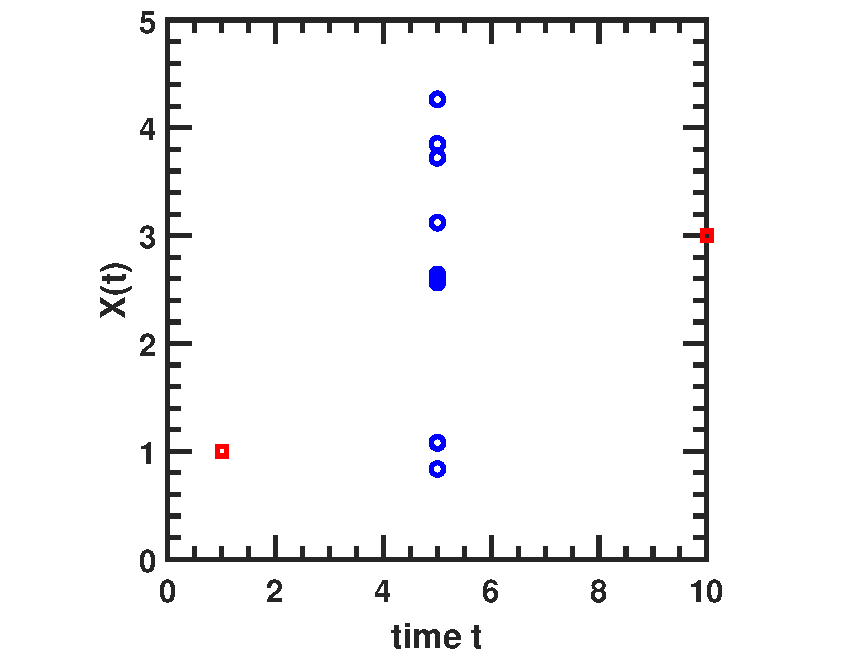
\includegraphics[width=\textwidth]{figures/stochasticProcess/monteCarlo/BrownianInterpolationDemo1}
		\caption{Brownian motion interpolation at a single time point.}
	\end{subfigure}\quad
	\begin{subfigure}[b]{0.4\textwidth}
		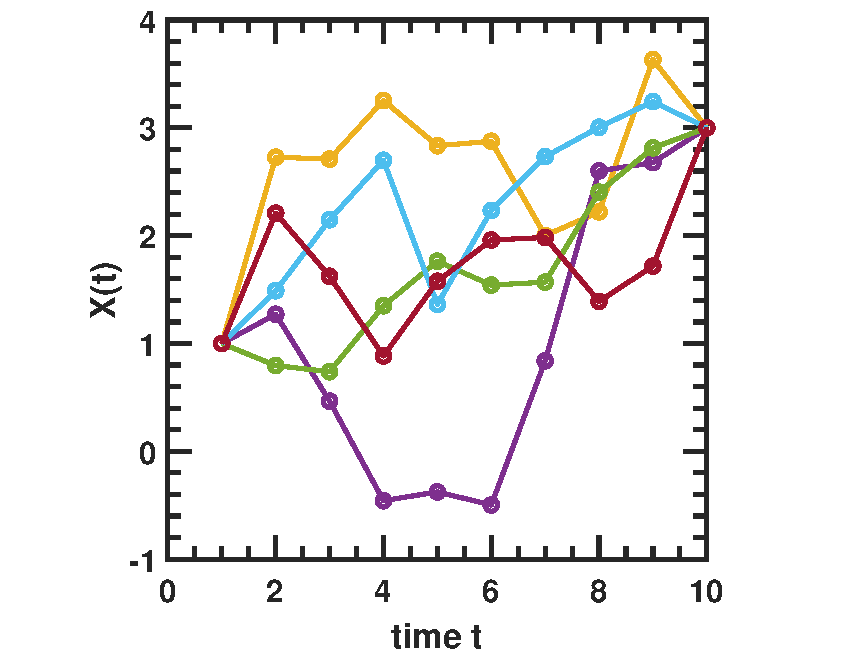
\includegraphics[width=\textwidth]{figures/stochasticProcess/monteCarlo/BrownianInterpolationDemo2}
		\caption{Brownian motion interpolation at multiple time points to generate trajectories.}
	\end{subfigure}
	\caption{Brownian motion interpolation Demo.}
	\label{ch:MonteCarlo-methods--optimization:fig:BrownianMotionInterpolationDemo}
\end{figure}

\subsubsection{Interpolating multi-dimensional Brownian motions}


\begin{lemma}[interpolating a standard multi-dimensional Brownian motion]
	Let $X(t) = (X_1(t),...,X_n(t))$ be a $n$-dimensional Brownian motion as the solution to an SDE governed by
	$$dX_i(t) = dW_i(t),i=1,2,...,n,$$
	where $E[dW_i(t)dW_j(s)] = \rho_{ij}\delta(s-t)$. 
 Let Cholesky decomposition of the instantaneous correlation matrix $\rho\in \R^{n\times n}$ be given by $\rho = DD^{T}$. Now consider three time points $t_a<t_1<t_b$. Then conditioning on values of $X(t_a)$ and $X(t_b)$,
	$X(t_1)$ is a Gaussian random variable with mean and variance $$\mu = X(t_a) + \frac{t_1-t_a}{t_b-t_a}(X(t_b)-X(t_a)), \Sigma = (t_1-t_a - \frac{(t_1-t_a)^2}{(t_b-t_a)})\rho.$$
\end{lemma}
\begin{proof}
Note that (\autoref{ch:theory-of-stochastic-process:def:MultiDimensionalCorrelationBrownianMotion}) the covariance matrix for $X(t)$ as $Cov(X(t),X(s)) =  \rho \min(s,t)$. 	
	
	Note that the random vector $(X(t_a), X(t_1),X(t_b))$ will follow multivariate Gaussian distribution. Conditioning on $X(t_a)$ and $X(t_b)$, $X(t_1)$ is a Gaussian random vector with conditional mean and variance given by(\autoref{ch:theory-of-statistics:th:multivariatenormalconditionaldistribution}) 
	\begin{align*}
	\mu&=[t_a \rho ~ t_1 \rho]\begin{bmatrix}
	t_a\rho & t_a\rho\\
	t_a\rho & t_b\rho
	\end{bmatrix}^{-1}\begin{bmatrix}
	X(t_a)\\
	X(t_b)
	\end{bmatrix} \\
	&= D [t_a  ~ t_1 ]\begin{bmatrix}
	D^T & 0\\
	0 & D^T
	\end{bmatrix}(\begin{bmatrix}
	D & 0\\
	0 & D
	\end{bmatrix}\begin{bmatrix}
	t_aI_n & t_aI_n\\
	t_aI_n & t_bI_n
	\end{bmatrix}\begin{bmatrix}
	D^T & 0\\
	0 & D^T
	\end{bmatrix})^{-1}\begin{bmatrix}
	X(t_a)\\
	X(t_b)
	\end{bmatrix} \\
	&= D [t_a  ~ t_1 ]\begin{bmatrix}
	t_aI_n & t_aI_n\\
	t_aI_n & t_bI_n
	\end{bmatrix}^{-1}\begin{bmatrix}
	D^{-1} & 0\\
	0 & D^{-1}
	\end{bmatrix}\begin{bmatrix}
	X(t_a)\\
	X(t_b)
	\end{bmatrix} \\
	&= DD^{-1}X(t_a) + \frac{t_1-t_a}{t_b-t_a}\rho(X(t_b)-X(t_a))\\
	&= X(t_a) + \frac{t_1-t_a}{t_b-t_a}\rho(X(t_b)-X(t_a))\\
	\end{align*}
	and
	variance
	\begin{align*}
	\sigma^2 &= t_1\rho - [t_a\rho ~ t_1\rho]\begin{bmatrix}
	t_a\rho & t_a\rho\\
	t_a\rho & t_b\rho
	\end{bmatrix}^{-1}\begin{bmatrix}
	t_a\rho \\
	t_1\rho
	\end{bmatrix} \\
	&=t_1\rho - D [t_a  ~ t_1](\begin{bmatrix}
	D & 0\\
	0 & D
	\end{bmatrix}\begin{bmatrix}
	t_aI_n & t_aI_n\\
	t_aI_n & t_bI_n
	\end{bmatrix}\begin{bmatrix}
	D^T & 0\\
	0 & D^T
	\end{bmatrix})^{-1}\begin{bmatrix}
	D & 0\\
	0 & D
	\end{bmatrix}\begin{bmatrix}
	t_a \\
	t_1
	\end{bmatrix}D^T \\
	&= D(t_1-t_a - \frac{(t_1-t_a)^2}{(t_b-t_a)})D^T\\
	&= (t_1-t_a - \frac{(t_1-t_a)^2}{(t_b-t_a)})\rho
	\end{align*}
\end{proof}


\begin{method}[sequential interpolating a multidimensional Brownian motion]
	Let $X(t)$ be a n dimensional Brownian motion with instantaneous correlation $\rho\in \R^{n\times n}$. Consider time points $t_a<t_1<t_2<\cdots < t_n<t_b$. Then conditioning on values of $X(t_a)$ and $X(t_b)$, we can sample $X(t_1),X(t_2),...,X(t_n)$ \textbf{as one sample trajectory} in the following way:
	\begin{itemize}
		\item sample $X(t_1)$ as a Gaussian random variable  with mean and variance $$\mu = X(t_a) + \frac{t_1-t_a}{t_b-t_a}\rho(X(t_b)-X(t_a)), \sigma^2 = (t_1-t_a - \frac{(t_1-t_a)^2}{(t_b-t_a)})\rho.$$
		\item sample $X(t_2)$ as a Gaussian random variable  with mean and variance $$\mu = X(t_1) + \frac{t_2-t_1}{t_b-t_1}\rho(X(t_b)-X(t_1)), \sigma^2 = (t_2-t_1 - \frac{(t_2-t_1)^2}{(t_b-t_1)})\rho.$$
		\item sample $X(t_i),i=3,4,...,n$ as a Gaussian random variable  with mean and variance $$\mu = X(t_{i-1}) + \frac{t_i-t_{i-1}}{t_b-t_{i-1}}\rho(X(t_b)-X(t_{i-1})), \sigma^2 = (t_i-t_{i-1} - \frac{(t_i-t_{i-1})^2}{(t_b-t_{i-1})})\rho.$$
	\end{itemize}
\end{method}
\begin{proof}
	Note that we use conditional independence such that $X(t_i)$ is indpendence of $X(t_{i-2})$ when conditioning on $X(t_{i-1})$.
\end{proof}


\section{Monte Carlo integration}\index{Monte Carlo}\index{Monte Carlo integration}


\subsection{Classic approach}
\begin{definition}
	The Monte Carlo integration refers to using
	$$\mean{h}_M = \frac{1}{M}\sum_{i=1}^M h(X_i)$$
	to approximate the integral
	$$E[h(x)] = \int_\cX h(x)f(x)dx$$
	where $\cX$ is the sample space of random variable $X$, $f(x)$ is the pdf, and $X_1,...,X_M$ are random samples of size $M$.
\end{definition}

\begin{example}[probability estimation]
	Probability estimation using $g(\theta) = 1(\theta\in \theta_0)$ which calculates the probability of $P(\theta\in \theta_0)$
\end{example}



\begin{lemma}[properties of approximation]\cite{andrieu2003introduction}\hfill
	\begin{itemize}
		\item The estimator is unbiased: $I_N(h) = E[\mean{h}_M] = I_h$;
		\item $\mean{h}_M $ converges to $I_h$ almost surely.
		\item The error distribution $$\sqrt{N}(\mean{h}_N - I_h)\sim N(0,\sigma_f^2) ~as~ N \to \infty,$$ where $\sigma^2_f = E[(\mean{h}_N - I_h)^2] = E[\mean{h}_N^2] - I_h^2$
	\end{itemize}
\end{lemma}
\begin{proof}
	(1) Linearity of expectation; (2) Strong law of large numbers\autoref{ch:theory-of-probability:th:stronglawlargenumber}; (3) Central limit theorem.
\end{proof}


\begin{remark}[pros and cons of Monte Carlo integration]\hfill
	\begin{itemize}
		\item Ordinary numerical integration over $n$ dimensions requires $~O(m^n)$ if $m$ is the number of divisions on each axis.
		\item Monte Carlo converges with speed $1/\sqrt{N}$ in standard deviation no matter how large dimensionality of the integral domain is.
	\end{itemize}
\end{remark}



\subsection{Importance sampling}\index{importance sampling}
\label{ch:MonteCarlo-methods--optimization:sec:importanceSampling}
\begin{algorithm}[H]
	\SetAlgoLined
	\KwIn{the proposal distribution $q(x)$ and the target distribution $p(x)$, the number $n$ of samples required, and the function $f(x)$ to be integrate}
	Sample $x\sim q(x)$ and calculate the corresponding weight $w(x) = p(x)/q(x)$\\
	Goto step 1 until $n$ samples are collected.\\
	Evaluate 
	$$I(f) = \int_{\cX} f(x) p(x)dx = \frac{1}{n}\sum_{i=1}^n f(x^i)w^i $$
	
	\KwOut{The sequence of sample pair$(x^1,w^1),...(x^n,w^n)$, and evaluted result}
	\caption{Importance sampling for integration }
\end{algorithm}

\begin{remark}
	Reference \cite{andrieu2003introduction}.
\end{remark}

\begin{lemma}[property of estimator]
	Let $I_n = \frac{1}{n}\sum_{i=1}^n f(x^i)w^i$, then we have
	\begin{itemize}
		\item The approximiation is unbiased: $$E_q[\frac{1}{n}\sum_{i=1}^n f(x^i)w^i] = \int_{\cX} f(x) p(x)dx = I(f) $$
		where $w(x) = p(x)/q(x)$.
		\item $I_n$ converges to $\int_{\cX} f(x) p(x)dx$ almost surely as $n\to \infty$.
	\end{itemize}
	
\end{lemma}
\begin{proof}
	(1) use linearity of expectation:
	\begin{align*}
	E[\frac{1}{n}\sum_{i=1}^n f(x^i)w^i] &= E[f(x)w(x)] = \int_{\cX} f(x)w(x)q(x)dx = E[f(x)w(x)]\\
	& = \int_{\cX} f(x)p(x)/q(x)q(x)dx = \int_{\cX} f(x)p(x)dx
	\end{align*}
	(2) Use strong law of large number (\autoref{ch:theory-of-probability:th:stronglawlargenumber}).Let $X_i = f(x^i)w^i = f(x^i)p(x)/q(x)$, then $E_q[X_i] = \mu = \int_{\cX} f(x)p(x)dx$. 
\end{proof}

\begin{lemma}[optimal proposal distribution]\cite{andrieu2003introduction}\cite[95]{robert2013monte}\cite{mcbook}
	In the importance sampling for Monte Carlo integration, we have
	$$I(f) = E_{p(x)}[f(x)] = E_{q(x)}[f(x)w(x)]$$
	where $w(x) = p(x)/q(x)$.
	The variance of $f(x)w(x)$ with respect to $q(x)$ is given by
	$$Var_{q(x)}[f(x)w(x)] = E_{q(x)}[f^2(x)w^2(x)] - I^2(f)$$
	And the variance has the lower bound
	$$E_{q(x)}[f^2(x)w^2(x)] \geq (E_{q(x)}[\abs{f(x)}w(x)])^2$$
	and the equality is achieved at 
	$$q^*(x) = \frac{\abs{f(x)}w(x)}{\int \abs{f(x)}w(x) dx}$$
\end{lemma}
\begin{proof}
	Note that $E_{p(x)}[f(x)]$ is unbiased estimator of $I(f)$. 
\end{proof}


\begin{remark}[interpretation]
	Good sampling estimates can be achieved when we focus on sampling region from $p(x)$ where $\abs{f(x)}p(x)$ is relatively large.
\end{remark}

\begin{remark}[convergence rate and optimal proposal distribution]
	Note that the optimal choice of the proposal distribution will not affect the convergence rate(still $1/\sqrt{N}$ in standard deviation), but will affect the prefactor.
\end{remark}



\begin{example}[tail probability estimation]\cite[93]{robert2013monte}
	Suppose $Z\sim N(0,1)$ and we want to estimate the tail probability as the integral of
	$$I = P(Z > 4.5) \approx \frac{1}{M}\sum_{i=1}^M I(Z^i>4.5)$$
	If we have proposal distribution $q(z) = e^{-(x-4.5)}/\int_{4.5}^\infty e^{-x}dx$, then 
	$$I = P(Z > 4.5) \approx \frac{1}{M}\sum_{i=1}^M I(Z^i>4.5) f(Z^i)/q(Z^i)$$
	where $f(z)$ is the pdf of $N(0,1)$.
	In this importance sampling scheme, we can collect much more samples in regions $Z>4.5$, but we will discount the sample contribution by the factor of $f(Z^i)/q(Z^i) $.
\end{example}



\begin{example}[pricing out-of-money call]
	Consider we price a call $E_Q[\max(S_T-K,0)]$. If $K$ is far from the mean value of $S_T$, then using Monte Carlo method will result in large variance. We can reduce the variance using importance sample via a proposal normal distribution with mean located near $K$.
\end{example}


\section{Monte Carlo variance reduction}\index{variance reduction}
\subsection{Antithetic sampling}
\subsubsection{Basic principles}
\begin{definition}[antithetic variates]\index{basic antithetic variates}\hfill
	\begin{itemize}
		\item Let $X$ be a random variable $X\sim U(0,1)$, then $1-X$ is also $U(0,1)$.
		\item Let $Y$ be a standard normal random variable $N(0,1)$, then $-Y$ is also $N(0,1)$ random variable.  
		\item Let $Z$ be a  normal random variable $N(\mu,\sigma^2)$, then $2\mu-Z$ is also $N(\mu,\sigma^2)$ random variable. 
	\end{itemize}
	The pairs $X$ and $1-X$ or $Y$ and $-Y$ are called \textbf{antithetic variates}. 
\end{definition}

\begin{remark}[negative correlation between antithetic variate pairs]
	The most important property of antithetic variates is that each pair is negatively correlated. For example, $X$ and $1-X$; $Y$ and $-Y$.
\end{remark}


\begin{theorem}[preserving negative correlation via monotone function]\cite[209]{ross2013simulation}\label{ch:MonteCarlo-methods--optimization:th:preservingnegativecorrelationsviamonotonefunction}
	If $h(x_1,...,x_n)$ is a monotone function of each of its arguments, then for a set of independent uniform random variables $U_1,...,U_n$, 
	$$Cov[h(U_1,...,U_n),h(1-U_1),...,1-U_n]\leq 0.$$
	Similarly, if $Z_1,...,Z_n$ is a set of independent standard Gaussian random variables, then
	$$Cov[h(Z_1,...,Z_n),h(1-Z_1),...,1-Z_n]\leq 0.$$
\end{theorem}
\begin{proof}
	See reference.
\end{proof}

\begin{lemma}[preserving negative correlation via linear function]
	Let $X,\hat{X}$ be two iid random variables and negatively correlated,i.e., $Cov(X,\hat{X}) < 0$. Let $f(x)=ax+b$ be a linear function, then
	$$Cov(f(X),f(\hat{X}))  < 0.$$
\end{lemma}
\begin{proof}
	$$Cov(f(X),f(\hat{X})) = a^2 Cov(X,\hat{X}) < 0.$$
\end{proof}

\begin{lemma}[generating antithetic variates of other distributions]\cite[205]{glasserman2003monte}
	Let $F$ be the cdf of the target distribution, let $F^{-1} = \inf\{F^{-1}(x>u)\}$. Then
	\begin{itemize}
		\item $F^{-1}$ is a monotone function.
		\item $F^{-1}(U)$ and $F^{-1}(1-U)$ are a pair antithetic variates with negative correlations.
	\end{itemize}
\end{lemma}
\begin{proof}
	(2) use \autoref{ch:MonteCarlo-methods--optimization:th:preservingnegativecorrelationsviamonotonefunction}.
\end{proof}

\subsubsection{Methods and analysis}
\begin{mdframed}
	\textbf{general principles}\\
	Let $S$ and $S'$ be a pair of antithetic variates random variables.  
	If $C = g(S)$ (where $g$ is a monotone function) is a calculation based on  $S$, then $C'=g(S')$ is negatively correlated with $C$ (\autoref{ch:stochastic-methods--optimization:th:preservingnegativecorrelationsviamonotonefunction}). 
\end{mdframed}

\begin{lemma}
	Considering $n$ iid random sample of $S$ and $n$ antithetic variate iid random sample of $S'$. Suppose we want to estimate the mean value of a function $C$,which is a monotone function of $S$. The estimator for the mean value is given as 
	$$\hat{C} = \frac{1}{2n}(\sum_{k=1}^n C_k + \sum_{k=1}^n C_k') = \frac{1}{n}\sum_{k=1}^n \frac{1}{2}(C_k' + C_k)$$ 
	Then 
	\begin{itemize}
		\item $\hat{C}$ is an unbiased estimator.
		\item $Var[C]$ is smaller than the variance of 2n sample mean estimator $C$; that is, using antithetic variates, smaller estimation variance can be achieved when using the same size of random samples. 
	\end{itemize}
\end{lemma}

\begin{proof}
	Note that the $n$ pairs of $ \frac{1}{2}(C_k' + C_k)$ are independent with each other. Moreover, $$\sigma^2( \frac{1}{2}(C_k' + C_k)) \leq \sigma^2(C_k)$$ since 
	$$\sigma^2( \frac{1}{2}(C_k' + C_k)) \leq \frac{1}{4}(\sigma^2(C_k) + \sigma^2(C_k') + 2cov(C_k,C_k')) \leq \frac{1}{2}\sigma^2(C_k)$$
	since $cov(C_k,C_k') \leq 0$.
	
	Therefore, when using the same number of random samples, antithetic variate samples can have a smaller variance on estimating the expectation.	
\end{proof}


\begin{remark}[caution!]
	Antithetic method can only be used to \textbf{estimate the expectation rather than the variance.}
\end{remark}

\begin{example}
	Suppose we want to estimate the mean value $f(X) = X^2, X\sim N(2,1)$. We can use the following estimator
	$$\frac{1}{n}\sum_{i=1}^n(f(X_i) + f(-X_i))/2.$$ 
	Note that even though $X^2$ is not a monotone function, it is nearly 'monotone' in regions where probability weight concentrates. 
\end{example}



\begin{example}[option pricing]\hfill
	\begin{itemize}
		\item Consider we simulate a Brownian motion by adding up random samples from $N(0,1)$. Let $C=\sum_{i=1}^n S_i$. Then the antithetic path is given as $C'=\sum_{i=1}^n -S_i$. These antithetic paths can be used to reduce variance of Monte Carlo method based option pricing.  
		\item Suppose we want to estimate $$C = E[e^{-rT}\max\{0,S_T-K\}],$$
		where $S_T = S_0e^{(r-\sigma^2/2)T+\sigma\sqrt{T}X},X\sim N(0,1)$. We can use standard normal antithetic variate to estimate $C$ to reduce variance since $S_T$ and $C$ are both monotone functions. 
	\end{itemize}
\end{example}

\begin{lemma}[variance reduction using normal random sample]\cite[208]{glasserman2003monte}
	Let $Y = f(Z)$  with $Z=(Z_1,...,Z_d) \sim N(0,1)$. Define the symmetric and antisymmetric parts of $f$, respectively, by
	$$f_0(z) = \frac{f(z) + f(-z)}{2}, f_1(z) = \frac{f(z) - f(-z)}{2}.$$
	We have
	\begin{itemize}
		\item $$E[f_0(Z)f_1(Z)] = 0, E[f_1(Z)] = 0,$$  $$Cov(f_0(Z),f_1(Z)) = E[f_0(Z)f_1(Z)] - E[f_0(Z)]E[f_1(Z)] = 0. $$
		that is $f_0(Z)$ and $f_1(Z)$ are not correlated.
		\item variance decomposition $$Var[f(Z)] = Var[f_0(Z)] + Var[f_1(Z)].$$
		\item $$Var[\frac{1}{2}(f_1(Z) + f_1(-Z)] = 0$$
		\item Antithetic sampling eliminates all variance if $f$ is antisymmetric($f=f_1$);It eliminates no variance if $f$ is symmetric($f=f_0$).
	\end{itemize}
\end{lemma}
\begin{proof}
	(1) $E[f_1(Z)] = 0$ because of $f_1(x) = -f(-x)$ and $Z$ is symmetric around $0$.
	$$E[f_0(Z)f_1(Z)] = \frac{1}{4}(E[f(Z)^2 + f(-Z)^2]) = 0$$
	because $Z$ is symmetric around $0$. 
	(2) use$$Var[X+Y]=Var[X]^2+Var[Y]^2 + 2Cov(X,Y).$$
	(3) Note that $f_1(Z) = - f_1(-Z)$. (4) Due to the variance decomposition in (2) and (3).
\end{proof}



\subsection{Control variates}\index{control variate}
\subsubsection{Basic principles}
\begin{mdframed}
	\textbf{General principles}\\
	The principle of control variates is to use estimation error of known quantities to improve the estimation of unknown quantities.\\
\end{mdframed}

\begin{lemma}\cite[188]{glasserman2003monte}
	Let $X_1,...,X_n$ be n samples of $X$, let $Y_1,...,Y_n$ be n samples of $Y$ with $E[Y]$ \textbf{known}. Then for any constant $\beta$, the statistic
	$$C(\beta) = \frac{1}{n}\sum_{i=1}^n( X_k - \beta(Y_k - E[Y]))$$
	is a control variate estimator for $E[X]$. Then 
	\begin{itemize}
		\item $C(\beta)$ is an unbiased estimator.
		\item its variance is given as
		$$Var[C(\beta)] = \frac{1}{n}(Var[X] - 2\beta cov(X,Y) + \beta^2Var[Y])$$
		\item If $\beta$ is chosen as 
		$$\beta = \frac{Cov(X,Y)}{Var[Y]}$$
		then $Var[C(\beta)] = Var[C] - \frac{Cov(X,Y)^2}{Var[Y]} \leq Var[C]$. The ratio of the variance is given as
		$$\frac{Var[C(\beta)]}{Var[C]} = 1 - \rho_{XY}^2$$
	\end{itemize}
\end{lemma}
\begin{proof}
	(1)(2) Straight forward. (3) do optimization on $\beta$. 
\end{proof}

\begin{remark}[interpretation]\hfill
	\begin{itemize}
		\item The working of this method relies on that there exist correlations between two random variables.  
		\item The amount of the variance reduction depends on the correlation coefficients of $X$ and $Y$. From (3), if $X$ and $Y$ is uncorrelated, then zero reduction can be achieved; if perfectly correlated, we can achieve complete reduction. 
	\end{itemize}
\end{remark}





\begin{remark}[practical calculation of $\beta$]
	Note that the optimal $\beta$ requires calculation of $Cov(X,Y)$(and $E[X]$), which might not be available. But we can estimate them from the simulation experiment itself. For example,
	$$\hat{\beta} = \frac{\sum_{i=1}^n (X_i - \mean{X})(Y_i - \mean{Y})}{\sum_{i=1}^n (Y_i - \mean{Y})^2}.$$
\end{remark}

\begin{example}[underlying asset as control variate for derivative pricing]\cite[188]{glasserman2003monte} Consider an option on underlying asset $S(t)$. We know that $e^{-rt}S(t)$ is a martingale and $$E[e^{-rt}S(t)] = S(0).$$
	Let the \textbf{discounted} payoff of the option be $Y$, then the control variate estimator for the price will be
	$$\frac{1}{n}\sum_{i=1}^n (Y_i - \beta(S_i(T) - e^{rT}S(0)).$$
	Consider the case that $Y = e^{-rT}\max(S(T)-K,0)$. Then the effectiveness of variance reduction depends on the correlation and $Y$ and $S$, which further depends on the value of $K$. If $K = 0$, then we have perfect correlation to achieve large reduction; if $K$ is large, then the correlation will be small.
\end{example}



\subsubsection{Multiple control variates}

\begin{lemma}\cite[196]{glasserman2003monte}
	Suppose each replication $i$ of a simulation produces outputs $Y_i $ and $X_i = (X_1^{(1)},...,X_i^{(d)})^T$ and suppose the vector of expectations $E[X]$ is known. We assume the covariance matrix $Cov(X,Y)$ is known as
	$$\begin{bmatrix}
	\Sigma_X & \Sigma_{XY}\\
	\Sigma_{XY} & \sigma_Y^2
	\end{bmatrix}$$
	Then the estimator of $Y$ via multiple control variates are given 
	$$\hat{Y}(\beta) = \frac{1}{n}\sum_{i=1}^n (Y_i - \beta^T (X_i - E[X]))$$
	where $\beta\in \R^d$. 
	We have 
	\begin{itemize}
		\item $E[\hat{Y}(\beta)] = E[Y]$.
		\item The variance of $\hat{Y}(\beta)$ is
		$$Var[\hat{Y}(\beta)] = \frac{1}{n}(\sigma^2_Y - 2\beta^T\Sigma_{XY} + \beta^T\Sigma_{X}\beta).$$
		\item The optimal $\beta$ achieving minimal variance is
		$$\beta^* = \Sigma_X^{-1}\Sigma_{XY},$$
		with the minimum variance given as
		$$\sigma_Y^2 - \Sigma_{XY}^T \Sigma_X^{-1}\Sigma_{XY}.$$
	\end{itemize}
	
\end{lemma}
\begin{proof}
	Straight forward.
\end{proof}



\begin{example}[multiple control variates]\hfill
	\begin{itemize}
		\item When we price a derivative that involves $d$ underlying assets, then the $d$ assets simulated results can provide control variates. 
	\end{itemize}	
	
\end{example}










\section{Markov chain Monte Carlo }\index{Markov chain Monte Carlo}


\begin{definition}[Markov chain Monte Carlo]
	Markov chain Monte Carlo(MCMC) methods are a class of algorithms to draw samples from a probability distribution $P$ by construct and simulate an \textbf{irreducible and aperiodic Markov chain} that has the  desired distribution $P$ as the equilibrium distribution of the chain.   
\end{definition}

\begin{remark}[interpretation]\hfill
	\begin{itemize}
		\item If the target distribution $P$ is simple (e.g. one dimensional)and known, we can just use method in \autoref{ch:stochastic-methods--optimization:sec:generateRN}.
		\item MCMC is particularly useful \textbf{if we only know the local conditional distribution, and we want to construct the global joint distribution.} For example, for a linear chain graphic model of $X_1,...,X_n$, we only know $P(X_{j+1}|X_j)$, then we can use MCMC to generate samples from $P(X_1,...,X_n)$.  
	\end{itemize}
\end{remark}

\subsection{Metropolis-Hasting algorithm}\index{Metropolis-Hasting algorithm}

\begin{algorithm}[H]
	\SetAlgoLined
	\KwIn{Initial state $x_0\in \R^d$, $p(x)$ known upto the scale, and number of sampling steps}
	Given a previous state $x$, sample a new state $x'$ based on \textbf{proposal distribution} $g(x'|x)$, a conditional distribution parameterized by two parameters $x$ and $x'$ .\\
	Accepting the new state $x'$ based on \textbf{accepting ratio function}, parameterized by two parameters $x$ and $x'$, $A(x'|x)$. One common choice of accepting ratio function is the Metropolis choice, given as
	$$A(x'|x) = \min(1,\frac{P(x')}{P(x)}\frac{g(x|x')}{g(x'|x)})$$\\
	Go to step 1 until $n$ samples are collected.\\
	\KwOut{The full sequence of sampled states $x_0,x_1,...$The low dimensional coordinate $y_i \in \R^p,i=1,2,...,N$}
	\caption{Metropolis-Hasting algorithm}
\end{algorithm}


\begin{remark}[knowing $P(x)$ is necessary]
	To execute the algorithm, we have to know $P(x)$ up to scale; otherwise $A(x'|x)$ cannot be determined.For example, in Ising model of statistical physics, we have $P(x) \sim \exp(-U(x)/kT),x\in \R^{2N}$ based on Boltzmann distribution.
\end{remark}




\begin{lemma}[transition probability and detailed balance]
	In the Metropolis-Hasting algorithm, the transition probability is given as
	$$P(x'|x) = g(x'|x)A(x'|x)$$
	and detailed balance are satisfied between any pair of states when use Metropolis accepting ratio, that is
	$$P(x'|x)P(x) = P(x|x')P(x')$$	
\end{lemma}
\begin{proof}
	(1) directly from the definition of proposal distribution and accepting ratio function; (2) 
	$$\frac{A(x'|x))}{A(x|x')} = \frac{\min(1,\frac{P(x')}{P(x)}\frac{g(x|x')}{g(x'|x)})}{\min(1,1/\frac{P(x')}{P(x)}\frac{g(x|x')}{g(x'|x)})}$$
	Note that if $$\frac{P(x')}{P(x)}\frac{g(x|x')}{g(x'|x)} >1,$$ we have 
	$$\frac{A(x'|x))}{A(x|x')} = \frac{P(x')}{P(x)}\frac{g(x|x')}{g(x'|x)},$$
	which implies detailed balance given by
	$$P(x)g(x'|x)A(x'|x)=P(x'|x)P(x) = P(x|x')P(x') = P(x')g(x|x')A(x|x')$$
	
	If $$\frac{P(x')}{P(x)}\frac{g(x|x')}{g(x'|x)} \leq 1$$ we get the same conclusion.
\end{proof}

\begin{theorem}
	The Metropolis-Hasting algorithm is constructing and sampling a Markov chain having an unique stationary distribution $P(x)$.
\end{theorem}
\begin{proof}
	Note that the chain construct will satisfy detailed balance, and we can use \autoref{ch:markov-chains:th:detailedbalance}
\end{proof}


\subsection{Biased MCMC: umbrella sampling}


\begin{algorithm}[H]
	\SetAlgoLined
	\KwIn{Initial state $x_0\in \R^d$, $p(x)$ known upto the scale, the biasing function $w(x)$, and number of sampling steps}
	Given a previous state $x$, sample a new state $x'$ based on \textbf{proposal distribution} $g(x'|x)$, a conditional distribution parameterized by two parameters $x$ and $x'$ .\\
	Accepting the new state $x'$ based on \textbf{accepting ratio function}, parameterized by two parameters $x$ and $x'$, $A(x'|x)$. One common choice of accepting ratio function is the Metropolis choice, given as
	$$A(x'|x) = \min(1,\frac{P(x')w(x')}{P(x)w(x)}\frac{g(x|x')}{g(x'|x)})$$\\
	Go to step 1 until $n$ samples are collected.\\
	Construct empirical distribution $p'(x)$ from the samples.\\
	Correct to correct distribution via $p(x) = p(x)'/w(x)$.\\ 
	\KwOut{The corrected distribution $p(x)$.}
	\caption{Umbrella sampling for probability estimation}
\end{algorithm}


\begin{remark}
	Reference \cite{kastner2011umbrella}
\end{remark}

\begin{remark}
	By choosing $w(x)$ to put larger value on low probability region, we have able to generate samples on these low probability region.
\end{remark}



\subsection{Gibbs sampling}

\begin{algorithm}[H]
	\SetAlgoLined
	\KwIn{Initial state $x_0 \in \R^d$, $p(x_i|x_{-i})$, and number of sampling steps}
	Given a previous state $x^{s-1}$, sample a new state $x^{s}$ using the following procedure:
	\begin{itemize}
		\item sample $x^{s}_1 \sim p(x^s_1|x_2^{s-1} ... x_d^{s-1})$
		\item sample $x^{s}_2 \sim p(x^s_2|x_1^s,x_3^{s-1} ... x_d^{s-1})$
		\item $\dots$
		\item sample $x^{s}_d \sim p(x^s_1|x_1^s ... x_{d-1}^{s})$
	\end{itemize}
	Go to step 1 until $n$ samples are collected.\\
	\KwOut{The full sequence of sampled states $x_0,x_1,...$}
	\caption{Gibbs sampling algorithm}
\end{algorithm}

\begin{lemma}[conditional independence property of sample]
	Given the sequence $x^1,x^2,...,x^n$ samples from Gibbs sampling procedure, we have
	\begin{itemize}
		\item The samples are dependent on each other. 
		\item $x^s$ is conditionally independent of $x^1,...,x^{s-2}$ given $x^{s-1}$.
	\end{itemize}
	
\end{lemma}
\begin{proof}
	Note that $x^s$ depends on $x^1,...,x^{s-2}$ only through $x^{s-1}$. From the perspective of graphical model, the sample generation form a chain structure. See \autoref{ch:theory-of-statistics:sec:graphical-models}.
\end{proof}

\section{Monte Carlo estimation of derivatives}

\begin{definition}[setup]\hfill
\begin{itemize}
	\item Suppose we want to estimate the derivative of a function $V(\sigma, Y)$ with resepct to a parameter $\sigma$.
	\item $V(\sigma, Y)$ is a function of both $\sigma$ and the \textbf{random variable }$Y$, where $Y$ is generated via directly sampling on its distribution $f_Y$ or via trajectory $X_0, X_1,...,X_N = Y$ simulated by MCMC. 
	\item Denote $\hat{V}(\sigma, X_N, s, M)$ as the Monte Carlo estimator using seed vector $s\in \N^M$ and $M$ trajectories, defined by
	$$\hat{V} = \frac{1}{M} \sum_{i=1}^M V(\sigma, y_i(s_i)),$$
	where $y_i$ denotes the $i$th realization of $Y$.
\end{itemize}	
\end{definition}


\begin{lemma}[bias and variance of finite difference scheme ]\href{https://quant.stackexchange.com/questions/3329/how-to-get-greeks-using-monte-carlo-for-arbitrary-option}{link}\cite[385]{glasserman2003monte}
Consider using \textbf{the same seed vector} $s$ in evaluating $\hat{V}(\sigma, X_N, s, M)$ and its perturbation. 
\begin{itemize}
	\item The forward difference scheme $$\hat{\Lambda} = \frac{\hat{V}(\sigma+\Delta \sigma, X_N, s, M) - \hat{V}(\sigma-\Delta \sigma, X_N, s, M) }{2\Delta \sigma}$$
	is a \textbf{biased estimator} (bias is due to finite difference scheme) such that
	 $$Bias = E[\hat{\Lambda} - \Pa V /\Pa \sigma] = O(\Delta \sigma),$$
	 and
	 variance (variance is due to finite sampling)
	 $$Var[\hat{\Lambda}] \approx \frac{2}{\Delta \sigma} Var[\hat{V}(\sigma, X_N, s, M)];$$
	 The total 
\end{itemize}




Moreover, assuming central limit theorem holds, the variance of the stimator is given by
	
\end{lemma}
\begin{proof}
(1)	
 By using the same seed, we have
\begin{align*}
\hat{\Lambda} &\triangleq \frac{1}{M \Delta \sigma}\sum_{i=1}^N(V(\sigma + \Delta \sigma, x_i) - V(\sigma - \Delta \sigma, x_i)) \\
&=\frac{1}{\Delta \sigma} (\frac{1}{M }\sum_{i=1}^M(V(\sigma + \Delta \sigma, x_i)) - (\frac{1}{M }\sum_{i=1}^M (V(\sigma - \Delta \sigma, x_i)) \\
&=\frac{\hat{V}(\sigma+\Delta \sigma, X_N, s, M) - \hat{V}(\sigma-\Delta \sigma, X_N, s, M) }{2\Delta \sigma}
\end{align*}
(2)
\end{proof}



\begin{note}[interpretation]\hfill
\begin{itemize}
	\item (\textbf{importance of controlling the seed})
	\item (error sources of derivative estimator)
\end{itemize}
\end{note}



\begin{method}
	
	
	$$\Lambda^{(1)} = \frac{\hat{V}(\sigma+\Delta, X_N, s, M) - \hat{V}(\sigma-\Delta, X_N, s, M) }{2\Delta \sigma},$$
	$$\Lambda^{(1)} = \frac{\hat{V}(\sigma+\frac{1}{2}\Delta \sigma, X_N, s, M) - \hat{V}(\sigma-\frac{1}{2}\Delta \sigma, X_N, s, M) }{\Delta \sigma},$$
	
	such $\abs{\Lambda^{(1)} - \Lambda^{(2)}} < tol$.
\end{method}



\subsection{Path-dependent derivatives}

\begin{lemma}[asset trajectory derivative with respect to spot]\cite[391]{glasserman2003monte}
\begin{itemize}
	\item Assume $S(t)$ is governed by SDE given by
	$$\frac{dS(t)}{S(t)} = \mu(t)dt + \sigma(t)dW(t),$$
	in which $\mu(t)$ and $\sigma(t)$ could be stochastic but have no dependence on $S(0)$. Then the asset price at $T$ is
	$$S(T) = S(0)\exp(\int_{0}^{T}(\mu(t)-\frac{1}{2}\sigma^2(t))dt + \int_0^T\sigma(t)dW(t));$$
	and
	$$\frac{dS(T)}{dS(0)} = \frac{S(T)}{S(0)}.$$
	\item In general, if $S(T) = S(0)\exp(X(T))$ for some (stochastic) process $X(t)$ that does not depend on $S(0)$, then
	$$\frac{dS(T)}{dS(0)} = \frac{S(T)}{S(0)}.$$
\end{itemize}	
\end{lemma}
\begin{proof}
(1)(2) $$\frac{dS(T)}{dS(0)}=X(T) = \frac{S(T)}{S(0)}.$$
\end{proof}


\begin{lemma}[path-dependent delta]\cite[389]{glasserman2003monte}
Consider an Asian option 
$$Y = \exp(-rT)(\mean{S} - K)^+, \mean{S} = \frac{1}{m}\sum_{i=1}^m S(t_i),$$
for some fixed dates $0 < t_1 < \cdots < t_m \leq T$.
Then the pathwise estimator of the option delta is
$$\frac{dY}{dS(0)} = \exp(-rT)\bm{1}(\mean{S}>K)\frac{\mean{S}}{S(0)}$$	
\end{lemma}
\begin{proof}
$$\frac{dY}{dS(0)} = \frac{dY}{d\mean{S}}\frac{d\mean{S}}{dS(0)} = \exp(-rT)\bm{1}(\mean{S}>K)\frac{d\mean{S}}{dS(0)}.$$
Also
$$\frac{d\mean{S}}{dS(0)} = \frac{1}{m}\sum_{i=1}^m \frac{dS(t_i)}{dS(0)} = \frac{1}{m}\sum_{i=1}^m \frac{S(t_i)}{S(0)} = \frac{\mean{S}}{S(0)}.$$

\end{proof}

\begin{lemma}[path-dependent vega]\cite[389]{glasserman2003monte}
	Consider an Asian option 
	$$Y = \exp(-rT)(\mean{S} - K)^+, \mean{S} = \frac{1}{m}\sum_{i=1}^m S(t_i),$$
	for some fixed dates $0 < t_1 < \cdots < t_m \leq T$.
	$$S(t_i) = S(t_{i-1})\exp((r-\frac{1}{2}\sigma^2)(t_i - t_{i-1} + \sigma \sqrt{t_i - t_{i-1}}Z_i), i = 1,...,m.$$
	Then the pathwise estimator of the option delta is
	$$\frac{dY}{dS(0)} = \exp(-rT)\bm{1}(\mean{S}>K)\frac{\mean{S}}{S(0)}$$	
\end{lemma}
\begin{proof}
	$$\frac{dY}{dS(0)} = \frac{dY}{d\mean{S}}\frac{d\mean{S}}{dS(0)} = \exp(-rT)\bm{1}(\mean{S}>K)\frac{d\mean{S}}{dS(0)}.$$
	Also
	$$\frac{d\mean{S}}{dS(0)} = \frac{1}{m}\sum_{i=1}^m \frac{dS(t_i)}{dS(0)} = \frac{1}{m}\sum_{i=1}^m \frac{S(t_i)}{S(0)} = \frac{\mean{S}}{S(0)}.$$
	
\end{proof}
\section{Quasi-Monte Carlo}
\subsection{Basics}
\begin{definition}[discrepancy]\index{discrepancy}\cite[283]{glasserman2003monte} Given a collection $\cA$ of (Lebesgue measurable) subsets of $[0,1)^d$, the discrepancy of the point set $\{x_1,...,x_n\}$ relative to $\cA$ is
	$$D(x_1,...,x_n;\cA) = \sup_{A\in \cA} \abs{\frac{\abs{x_i\in A}}{n} - vol(A)}$$
	where $vol(A)$ denotes the volume(measure) of $A$. 
	Typical $\cA$ can be
	\begin{itemize}
		\item the collection of all rectangles in $[0,1)^d$ of the form 
		$$\prod_{j=1}^d [u_j,v_j), 0 \leq u_j < v_j \leq 1.$$
		\item the collection of all rectangles in $[0,1)^d$ of the form 
		$$\prod_{j=1}^d [v_j,u_j), 0 \leq u_j \leq 1.$$
		In this case, the discrepancy is known as the star discrepancy($D^*$).
	\end{itemize}
\end{definition}

\begin{remark}[interpretation]\hfill
	\begin{itemize}
		\item The discrepancy is the maximum/supremum error in integrating the indicator function of $A$ using the points $x_1,...,x_n$.
		\item Intuitively, the uniformly distributed of the sequence, the lower the integration error, or, discrepancy.
	\end{itemize}	
\end{remark}



\subsection{Integration Error Estimation}

\begin{theorem}[Koksma-Hlawka inequality]\cite[288]{glasserman2003monte}
	
	
	
	$$\abs{\frac{1}{n}\sum_{i=1}^n f(x_i) - \int_{[0,1]}^{d} f(u) du} \leq V(f)D^*(x_1,x_2,...,x_n)$$
\end{theorem}


\begin{remark}[practical usage]\hfill
	\begin{itemize}
		\item Koksma-Hlawka inequality has limited practical application in estimating the error because usually $V(f), D^*$ are difficult to calculate.
	\end{itemize}
\end{remark}


\begin{remark}[comparison with conventional pseudo-random number]
	\begin{itemize}
		\item Use convensional pseudo-random number for integration, we have
		$$\abs{\frac{1}{n}\sum_{i=1}^n f(x_i) - \int_{[0,1]}^{d} f(u) du} \leq z_{\delta/2} \frac{\sigma_f}{\sqrt{n}}$$
		with probability $1-\delta$, with $z_{\delta/2}$ being the $\delta/2$ quantile of the standard normal distribution.
		\item 
		Simulations which use quasi-random
		numbers can achieve faster convergence ($N^{-1}(\log N)^{s-1}$) and
		better accuracy than simulations using conventional
		pseudo-random numbers $O(1/N^{0.5})$.\cite[10]{niederreiter1992random}.
	\end{itemize}
\end{remark}


\section{Stochastic approximation and optimization}

\subsection{Simulated annealing}

\begin{algorithm}[H]
	\SetAlgoLined
	\KwIn{Initial state $x_0\in \R^d$, $p(x)$ known upto the scale, and number of sampling steps $N$, cooling scheme for $T$, proposal transition probability $q(x'|x)$}
	Initialize $x_0$,$i=0$ and set $T_0 = 1$\\
	\Repeat{ i = N}{
		Sample $x^i \sim q(x^i|x^{i-1})$\\
		Accept $x^i$ with probability 
		$$\min\{1,\frac{p(x^i)^{1/T_i} q(x^{i-1}|x^i))}{p(x^{i-1})^{1/T_i} q(x^{i}|x^{i-1}))}\}$$
		Set $T_{i+1}$ accordint to chosen cooling scheme.\\
		i=i+1
	}
	\KwOut{The full sequence of sampled states $x_0,x_1,...$The low dimensional coordinate $y_i \in \R^p,i=1,2,...,N$}
	\caption{Simulating annealing algorithm}
\end{algorithm}

\begin{remark}
	Reference \cite{andrieu2003introduction}\cite{spall2005introduction}.
\end{remark}

\section{Notes on bibliography}

Introductory level Monte Carlo methods, see \cite{dunn2011exploring}.
Intermediate level Monte Carlo methods, see \cite{kroese2013handbook}\cite{robert2013monte}\cite{spall2005introduction}\cite{mcbook}.

For an excellent review on MCMC, see \cite{andrieu2003introduction}.

For advanced Monte Carlo methods in financial applications, see \cite{jackel2002monte}.

For Quasi Monte Carlo methods, see \cite{niederreiter1992random}\cite{jackel2002monte}.
\printbibliography

\end{refsection}
